Now that we have a handle on the reactions of DM observable at collider experiments, we turn to a description of the searches and experimental constraints for DM at colliders, privileging LHC searches as they generally set the most stringent constraints. For a detailed description of the LHC and the ATLAS, CMS and LHCb experiments, we refer to~\cite{LHC2008,ATLAS2008,CMS2008}. %CD: blurb more? I'd say no. 
The first period of LHC running (2010-2012) at 7 and 8 TeV center-of-mass energy ($\sqrt{s}$) is termed Run-1, while the second period (2015-2018) is called Run-2. 
The categorization of these searches follows loosely the description of the benchmark models. We start describing searches for DM interacting through SM bosons~\ref{sec:results_ZHSearches}, then move to generic searches for signals with missing transverse momentum~\ref{sec:results_monoXSearches}, and outline the searches for complete models with DM candidates in Section~\ref{sec:results_SUSYSearches}. Throughout this chapter
%and in Section~\ref{sec:experimentalChallenges} %CD: removed in favour of sidebars
we will highlight the experimental challenges and the novel experimental techniques used to overcome them,
motivated by the strong interest in dark matter searches. 
We then conclude with searches for long-lived particles within models of DM in
Section~\ref{sec:results_LLPSearches}. %CD: need to rewrite this sentence, but the idea is: if we hadn't had DM as a motivation motivation we wouldn't have done this difficult stuff. 

\subsection{Searches for DM in interactions mediated by SM-boson}
\label{sec:results_ZHSearches}

The invisible decays of the Z and Higgs boson are the main direct targets of searches for SM-boson-mediated interactions between SM and DM particles, if the DM particle is lighter than half the mass of the boson. Above this region, Direct Detection experiments are generally more sensitive than collider experiments. 
%CD: do we need to answer "what if not"? No one seems to care, but one could maybe think of using monojet off-shell (tiny tiny region) and precision constraints for the off-shell region too, a la dijet. Main point for the moment: DD covers this region so we don't have to. 
In the SM, the Z boson can decay to a neutrino-antineutrino pair, while the Higgs boson decays into a pair of Z bosons each decaying to neutrinos. Additional decays of the Z and Higgs boson to particles beyond the SM modify the properties of the vector boson, such as width and couplings. 

%MonoZ

%CD only mentioning below because it's like a monophoton
%Simple (but somehow messy) explanation in https://cds.cern.ch/record/1750933/files/CERN-THESIS-2013-330.pdf, Hugo's student
%Hugo did it, unpublished: https://www-cdf.fnal.gov/physics/ewk/2007/ZnunuWidth/
%CDF direct: 466 pm 42
\textbf{Decays of the Z boson into invisible particles} can be constrained using the invisible Z width. It can be measured directly in Z decays in association with a photon emitted as initial state radiation. Events are selected containing a single photon, missing transverse momentum and no other sizable event activity. This selection is also used for identifying events from possible DM reactions at colliders.
%LEP combined: 503 $\pm$ 16 MeV
The total Z width has been measured indirectly at LEP~\cite{ALEPH:2005ab} leading to a measurement of the number of light neutrino families compatible with cosmology; if the partial widths of the decays into visible particles are subtracted from the total width, the invisible width can be measured to 499.1 $\pm$ 1.5 MeV~\cite{Patrignani:2016xqp}. 
%The precision of the indirect measurement is better than that of the direct measurement, due to the higher statistics and the relative ease of selection and background subtraction for the visible Z decays. %CD: omitted, no space
%The main systematic uncertainty in this case comes from the theoretical uncertainties in the simulation. CD: Carena seems to think it is an uncertainty on fast simulation
New physics effects modify direct and/or indirect Z width~\cite{Carena:2003aj}.
\begin{marginnote}[]
Direct and indirect Z width measurements must agree if the decay of the Z to a pair of invisible new particles is to be the main mechanism responsible for the deviation from the SM values. 
\end{marginnote}%CD: I think this is important to mention in the same sense as the caveats on the s-channel resonances, but it can be omitted
%in this case, an analysis of the mass of the system recoiling against the photon would provide a handle to distinguish between different BSM processes. %CD: omitted because this is possibly too handwavy but how can we summarize 4 pages of Carena in a sentence?
%Carena quantitative: At present, measurements at LEP and CHARM II are capable of constraining the left-handed Z\nu\nu-coupling, 0.45 <~ g_L <~ 0.5,  while the right-handed one is only mildly bounded, |g_R| <= 0.2.
The LEP precision measurements~\footnote{Bounds on Z to invisible decays obtained from LHC searches are not yet competitive~\cite{deSimone:2014pda}.}, as well as direct detection experiments, rule out the majority of the Z-mediated DM scenarios~\cite{Arcadi:2014lta,Escudero:2016gzx}. The LEP invisible width is well below the width one would expect if vector and axial vector models of DM were realized, for all couplings satisfying the relic density with a DM mass below 25 GeV. Direct detection experiments such as Xenon1T~\cite{Aprile:2017iyp} 
%CD: take figure 2 of Escudero:2016gzx and compare with the results of Aprile:2017iyp
rule out most of the other simplified model scenarios compatible with freeze-out relic density up to multi-TeV DM masses. 
%DM mass above 6 TeV for the vector couplings, while for axial the plot is truncated. 

%%MonoH

\textbf{Invisible decays of the H boson} within the SM only contribute to less than 0.1\% of the total decay width. For this reason, an observation of even a small contribution to the Higgs width from invisible particles would signal the presence of new physics phenomena that could be linked to DM if 2\mdm $< m_H$~\footnote{For the case of heavier DM particles, see Ref.~\cite{Djouadi:2011aa}.}. 

Pre-LHC constraints on the invisible Higgs width are derived from measurements of the ZH production channel at LEP in searches for new neutral Higgs-like bosons, where only the visible decays of the Z are observed. This is a common procedure to select events in LHC DM searches. %CD: need a number! 
It is not feasible to directly or indirectly measure the total and partial Higgs widths at a hadron collider and then extract the invisible contribution as done for the Z at LEP, as some of the decays (e.g. gluons and lighter quarks) have too large a background to be measured, the experimental resolution even for leptonic decays is large compared to the intrinsic Higgs SM width, and the kinematics of the ZH process is not fully determined as in lepton colliders. %CD: this is ambiguous also because I am not sure I fully understand the first and third points completely - need AB's help, page 2 of Dobrescu/Lykken. 
%Lykken/Dobrescu, 1210.3342: Total theoretical SM width/mass for H125: 3.2 * 10^-5 MeV, due to small Yukawa of b quark and suppression of WW*. From rates and couplings,  can extract upper and lower limits on the exotic Higgs branching fractions, which come from the upper/lower limit on the total width. This paper ignores exp uncertainties. 
%Wagner Dark Side of the Higgs boson: omit because we don't care about non-SM Higgses
%The width can be extracted from the lineshape in the low-background channel $Z \rightarrow ZZ \rightarrow 4l$, assuming a SM width. This is what CMS has done. 
%If one does not want to assume the SM width, one can still extract the width
%above 190 GeV where the experimental resolution is better. 
%what we want to see is a larger total width with less normalization because of the invisible decays
Instead, searches at the LHC either attempt to directly observe the invisible decays of the Higgs boson, or compare measurements with precise theoretical calculations of SM parameters, to reveal
%unearth? there are no worms in this article so we should change this word
discrepancies signaling new physics or indirectly place constraints on new physics phenomena. 
Higgs to invisible LHC searches using Run-1 and Run-2 data~\cite{Khachatryan:2016whc,Aad:2015pla} employ and combine the $qq \rightarrow H qq$, $qq \rightarrow VH$, $gg \rightarrow HZ$, $gg \rightarrow Hg$ Higgs production modes. 
%CD: This section is just CMS for now. Need to add ATLAS, but also cut as we're using too much space for this:
%https://atlas.web.cern.ch/Atlas/GROUPS/PHYSICS/PAPERS/HIGG-2015-03/fig_09.png
In all cases, in addition to a requirement of sizable missing transverse momentum, auxiliary visible objects are used to select the events. 
%Loop-induced signals are important. 
%For more info on importance and calculation of loops: 1605.08039, but we run out of citations and space
The events are divided in exclusive categories targeting specific production modes. The associated boson (VH) searches target the decays of Z bosons to electrons, muons light or heavy flavour quarks, while the W bosons can decay into light-flavour jets. 
The $qq \rightarrow H qq$ production mode is dominated by Vector Boson Fusion (VBF) processes, where the Higgs boson is produced in association with two hadronic jets that have a large pseudorapidity ($\eta$)
%CD: assume eta?
separation in the detector, and a large invariant mass. This topology is used to select events and discriminate between signal and background. 
%The large QCD backgrounds are suppressed by requiring that the missing transverse momentum recoils against the jets in the event. 
%If the missing transverse momentum was in the direction of the jets, there would be a chance of it coming from mismeasured jets. %CD: hmmm written this in a rush
The jet+MET search, described in more detail in the next section, is reinterpreted for the $gg \rightarrow Hg$ mode. 

%The upper limit on the invisible BR from Higgs decays is 25%. 
%ATLAS Abstract
%Direct searches for invisible Higgs boson decays in the vector-boson fusion and associated production of a Higgs boson with W/Z (Z ? ??, W/Z ? jj) modes are statistically combined to set an upper limit on the Higgs boson invisible branching ratio of 0.25. The use of the measured visible decay rates in a more general coupling fit improves the upper limit to 0.23, constraining a Higgs portal model of dark matter.
%%Precision
Precision measurements of the Higgs boson properties and the comparison with SM theory also play a role in constraining the possible contributions to new physics, as decays into invisible particles would reduce the SM Higgs production and decay coupling strengths~\cite{Khachatryan:2016vau,Englert:2011yb,Aad:2015pla}. 
%For the Higgs boson, the upper limit on the branching fraction to visible and/or invisible non-SM particles only using precision measurements is 34\%
%In case we want to say what limits these
%The main limitation for the measurement of the invisible width of the Higgs at the LHC is due to QCD uncertainties the Higgs production cross-section, which limits the sensitivity of these searches to roughly 10\% of the SM value. 

The most stringent observed upper limit on the fraction of invisible decays of the Higgs boson, combining direct and precision measurements is 23\%.
%What does it mean for Higgs portal models: DD is always better
In the case of light fermion DM with scalar couplings to the Higgs, direct detection experiment rule out most of the parameter space where the model can provide the measured relic density~\cite{Escudero:2016gzx,Djouadi:2011aa}. Due to the suppression of the cross-section for DD in the pseudoscalar case, the model is still not constrained around a small region for DM masses corresponding to half the Higgs mass and above. %CD: maybe we have to say why this is the case - essentially rates are too small, see paper by Plehn. 

\subsection{Generic searches for DM with missing transverse momentum}
\label{sec:results_monoXSearches}

%Sidebar (50 words minimum, 200 words maximum) briefly discussing a fascinating adjacent topic; insert below Literature Cited section, but indicate near which section in text the sidebar should be typeset
\begin{textbox}[!h]
\section{Details of \MET reconstruction and fake \MET rejection}
This is why this is important, this is 10 words. 
This is why this is important, this is 10 words. 
This is why this is important, this is 10 words. 
This is why this is important, this is 10 words. 
This is why this is important, this is 10 words. 
This is why this is important, this is 10 words. 
This is why this is important, this is 10 words. 
This is why this is important, this is 10 words. 
This is why this is important, this is 10 words. 
This is why this is important, this is 10 words. 
This is why this is important, this is 10 words. 
This is why this is important, this is 10 words. 
This is why this is important, this is 10 words. 
This is why this is important, this is 10 words. 
This is why this is important, this is 10 words. 
This is why this is important, this is 10 words. 
This is why this is important, this is 10 words. 
This is why this is important, this is 10 words. 
This is why this is important, this is 10 words. 
This is why this is important, this is 10 words. 
This is why this is important, this is 10 words. 
This is why this is important, this is 10 words. 

%\subsubsection{Missing transverse momentum}
%\label{sub:MET} 

%Main points:
%\begin{itemize}
%\item The measurement of \MET relies on the precise measurement of all reconstructed physics objects. 
%\item Some description of \MET significance may be needed, but it may also be too academic. 
%\item Fake \MET is rejected using quality cuts.  
%\item Pile-up needs specific techniques because of the soft terms. 
%\item \MET at the trigger level is the driving reason why we can't go lower, see next section.
%\end{itemize}

%from ooutline

%- Mismeasured MET (combining instrumental effects and beam/cosmics background)				
%	- CDF				
%		- beam background: exploit track pointing to jet and calorimeter layers				
%		- QCD: shitty method from Mario (extrapolation changing the veto)				
%	- LHC:				
%		- beam backgrounds: like CDF, more refined				
%			- can have a % of how many events would have been				
%		- QCD: matrix method a la SUSY				
%	- Other backgrounds (diboson, top)				
%		- Small so using MC				
%		- LHC has validation regions				
%			- check ttbar				

%Valerio's talk for relevant plots 
%https://indico.cern.ch/event/466934/contributions/2590281/attachments/1489278/2314178/20170706_EPS_DMatATLAS.pdf

%MET significance: in VBF CMS search
%For the 8 TeV dataset, an additional requirement is set on an approximate missing transverse energy significance variable S(Emiss) defined as the ratio of Emiss to the square root of the scalar sum of the transverse energy of all PF objects in the event [62]. Selected events are required to satisfy S(Emiss) > 4?GeV.


\end{textbox}

WIMP DM particles at colliders escape detection, and their observation requires one or more visible objects in the same event. Searches that only rely on this feature are for the most part model-agnostic, as they only need to detect an excess of missing transverse momentum left by the DM particles recoiling against SM objects, without making any extra assumption on the DM particles or on their production mechanism. Similar search strategies have been employed as center-of-mass energy and dataset size increased, from LEP to Tevatron to the most recent LHC searches~\cite{Fox:2011fx,Beltran:2010ww,Bai:2010hh}. A generic event selection for excesses of \MET also provides an inclusive sample for more targeted searches as it will be discussed in Chapter~\ref{sec:05_Future}. 

We begin this section by describing the LHC searches for missing transverse momentum in association with one or more hadronic jets. The jet+\MET search allows us to illustrate many of the techniques used in invisible particle searches, and it is one of the most powerful to constrain BSM-mediated simplified models of dark matter. We then move on to outlining searches using different associated objects, and continue with searches for visible mediators that are the consequences of the DM production mechanism. Finally, we compare and discuss the sensitivity of invisible DM and visible mediator searches at the LHC. 

\subsubsection{Searches with jets}
%monojet

%%CD: I am not sure I would want to read this summary of monojet search. But maybe I'm just jaded. Anyway, if we can, we should make it more interesting / give it a slightly different spin than just a plain description. 

%%Intro and event selection

Events containing invisible particles can be identified and selected at colliders if initial state radiation (ISR) is present. For $e^+e^-$ colliders, the most frequently radiated object is a photon, while for hadron colliders gluon radiation dominates. These searches have been called "Mono-X", where X is the radiated object, although the radiation of a single object is only the leading process in a SM-DM $s-$channel interaction~\cite{Haisch:2013ata}. For this reason, the most recent LHC searches for MET with jets~\cite{Sirunyan:2017jix,Aaboud:2017phn} allow for events containing more than one jet in the final state. Since the presence of highly energetic invisible particles would manifest as an excess of events with a significant \MET, the main observable for this search is the number of events in \MET \textit{signal regions}, either exclusive (in bins of \MET) or inclusive (considering all events above a given \MET threshold). 
The discovery of a signal originating from one of the benchmarks DM models presents different challenges, depending on the DM particle mass and boost. If the mediator is heavy, any light DM particle will receive a boost and appear as an excess in the tails of the SM \MET distribution. If instead the DM particle pair originates from a light mediator, of the same mass range as the Higgs boson, it will manifest itself at low \MET. The low \MET suffers from a much higher rate of both instrumental and SM backgrounds. As a consequence, it is impossible to record and store all events with a low-\MET for further analysis, since at the data-taking stage (within the \textit{trigger} and data acquisition systems) it is difficult to obtain further handles to discriminate signal and background, and the sensitivity to low-\MET signals is compromised. This challenge will be discussed further for both visible and invisible particle searches in Sec.~\ref{sub:twoBody}.

\begin{marginnote}[]
\entry{Trigger}{a detector system that decides which LHC collision events are to be recorded for physics analysis. For a description of the trigger systems of the ATLAS and CMS experiments, see ~\cite{Smith:2016vcs,Aaboud:2016leb,Khachatryan:2016bia}.}
\end{marginnote}

%and  QCD subprocesses matter - too much detail too little space https://cds.cern.ch/record/159861/files/198507018.pdf

%in OOutline we wanted to quote example numbers, but there is a lot of eyeballing
%>1000 GeV: EM10: 226+/-16 events predicted, 245 observed
%WIMP mdm 400, mmed 1000: 0.2 (eyeballed)*200 GeV  

%up to 3 jets with pT>30 GeV for ATLAS
Events are selected to enter the \MET signal regions if they contain at least one jet in the central region of the detector ($\eta<2.4$) with \pt $>$ 250 GeV (ATLAS) or \pt $>$ 100 GeV (CMS) and \MET $>$ 250 GeV (ATLAS) or \MET $>$ 200 GeV (CMS). This selection ensures that all events with these characteristics are recorded by the trigger system for further analysis. A lepton veto is used to suppress background from leptonically decaying W bosons. 
%CMS excludes taus, while ATLAS does not. Too much detail imo. 
QCD background where large \MET originates from mismeasured jets is rejected by requiring that the $\phi$ direction of the missing transverse momentum vector does not align with the direction of the four-momentum of the jets with the highest \pt (leading jets). The remaining QCD background estimated from data amounts to a maximum of 0.4\% of the total background. The large number of events containing fake \MET due to non-collision background (e.g. cosmic rays, beam-gas interactions, calorimeter problems), shown in Fig.~\ref{fig:fakeMET} is rejected with specific quality criteria discussed in the relative Sidebar.%Sidebar? Textbox?

\begin{figure}[!htpb]
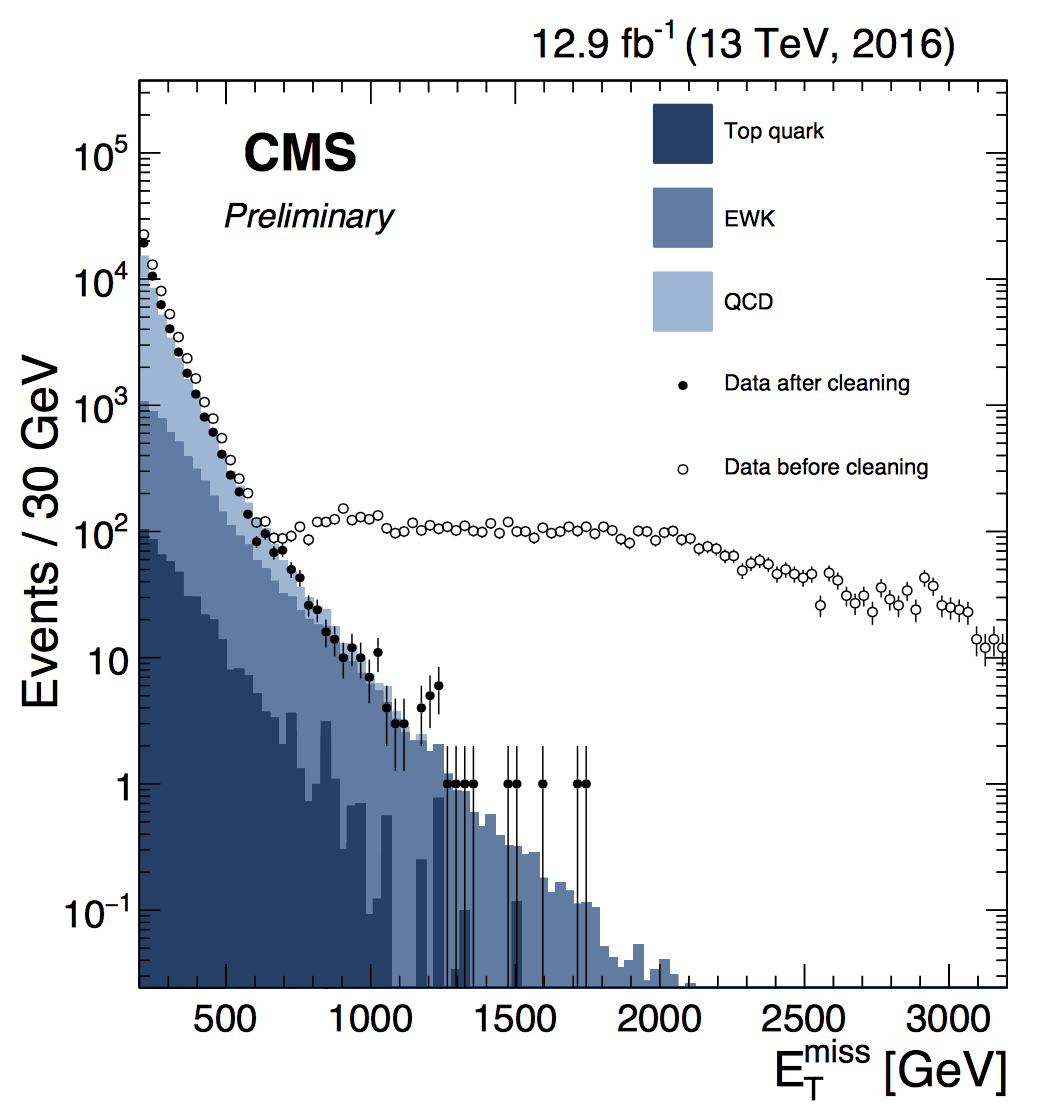
\includegraphics[width=0.5\textwidth]{figures/FakeMETTemp.png}
%Caption from the ATLAS monojet but they only have pT
%https://atlas.web.cern.ch/Atlas/GROUPS/PHYSICS/PAPERS/EXOT-2015-03/
\caption{The \MET distribution of the data events passing the [define selection] without any cleaning criteria applied on the leading jet. The Standard Model background indicated in the plots corresponds to the estimates obtained for the analysis signal region, including jet quality requirements. 
%The jet selection inefficiency of the cleaning selection is O(1\%), which is negligible compared to the observed excess in data. 
This demonstrates the necessity of a strong non-collision background suppression for this analysis. From~\cite{ToBeFound}.}
\label{fig:fakeMET}
\end{figure}

%CMS: up to 4 leading jets 
The CMS analysis also applies specific vetoes for photons and heavy flavour jets, to reject events with photon ISR or containing top quarks. The CMS analysis also includes a signal region targeting hadronic decays of the W and Z bosons using substructure techniques, which is considered separately in the case of ATLAS and will be discussed in Sec.~\ref{subsub:monoV}. 

\begin{marginnote}[]
\entry{Signal region}{a region of phase space for a search that is enriched in signal events. Event counts in this region are used to compare background-only prediction to data in search for discrepancies signaling new physics. 
%For example, a region with a high \MET and no other objects except for the ISR object is a signal region for a \MET+X search.
}
\entry{Control region}{a region of phase space for a search that is signal-free but with characteristics otherwise as close as possible to the signal region. Event counts in this region are used to estimate backgrounds in the signal region. 
%For example, a region requiring no \MET and a process mimicking that of the signal region is a control region for a \MET+X search.
}
\end{marginnote}


%%Backgrounds
The main background contributions that remain after the event selection are
invisible decays of the Z boson into neutrinos (approximately 55-70\% of the total background) 
%numbers in Livia's talk: https://indico.cern.ch/event/682235/contributions/2817876/attachments/1576792/2490208/DMWG-2017_V2.pdf and in Francesca's talk:
%https://indico.cern.ch/event/682235/contributions/2817877/attachments/1576793/2490236/171218_atlas_ungaro.pdf
and leptonic decays of the W boson where the lepton is not
reconstructed (approximately 20-35\% of the total background), in association with jets. 
%
In order to reduce theoretical and experimental uncertainties on the main V+jet backgrounds, the number of events in the signal region from each of these backgrounds are derived from data in signal-free \textit{control regions} selecting V+jet processes where the W and Z bosons decay into visible particles ($Z\rightarrow ll, W\rightarrow l\nu+jets$, where $l$ = $e, \mu$). 
%not sure we should say that the bin by bin estimates are used, here it's ambiguous
The event selection follows that of the signal region, substituting a lepton requirement to the lepton veto. The visible decay products in events selected for the control regions are subtracted from the total transverse momentum balance, providing an estimate of the contribution of these backgrounds in the signal region. CMS also uses a $\gamma$+jet control region where the photon is subtracted following the same procedure, to increase the statistical precision of the background estimate. 
%
The distribution of events in the main observable used for the search, the shape of the \MET distribution, is simulated and reweighted for each of the control regions using the most recent perturbative calculations for NLO QCD and QED~\cite{Lindert:2017olm}. The estimation of the number of $Z\rightarrow \nu\nu$events from the $\gamma$+jet and  $W\rightarrow l\nu$+jets control region needs a specific treatment due to the difference in the processes. This is particularly important for a consistent treatment of the different processes used in the background estimation and of the main theoretical uncertainties, and it will be discussed further in the following textbox. %CD: how do we call the thing
The full information on the theoretical and experimental uncertainties and their correlations from this procedure is used in a simultaneous fit to control and signal regions, to determine the overall background estimate in each of the \MET regions considered. 
%and leads to an improvement of 40 to 50% in the search according to PhilHarris and Livia, but I wouldn't add that unreferenced
Backgrounds from top processes in ATLAS are estimated using a dedicated control region with a requirement of a $b-$jet that is included in the fit, while CMS takes this background from simulation. Smaller diboson backgrounds are estimated from simulation. 

%Sidebar (50 words minimum, 200 words maximum) briefly discussing a fascinating adjacent topic; insert below Literature Cited section, but indicate near which section in text the sidebar should be typeset
\begin{textbox}[!h]
\section{Precision estimation of background for \MET+X searches}
In order to relate the number of events in the jet+\MET
signal regions (where $Z\rightarrow \nu\nu$ dominates) and control
regions (where events with jets produced in association with
$Z\rightarrow ll$, $W\rightarrow l\nu$ and $\gamma$ are used to maximise
the statistical power of the background estimation),
one needs to rely on a precise theory  
prediction of the ratio of the V+jets cross-sections. 
This is why this is important, this is 10 words. 
This is why this is important, this is 10 words. 
This is why this is important, this is 10 words. 
This is why this is important, this is 10 words. 
This is why this is important, this is 10 words. 
This is why this is important, this is 10 words. 
This is why this is important, this is 10 words. 
This is why this is important, this is 10 words. 
This is why this is important, this is 10 words. 
This is why this is important, this is 10 words. 
%\subsubsection{Precise background estimation}
%\label{sub:precision}

%Cite AR on this topi (but it's 2009): \cite{doi:10.1146/annurev.nucl.56.100704.122617}
%from ooutline
%- LHC results				
%	citations for most recent
%	- Differences between ATLAS and CMS:				
%		- CMS starts with only Z, ATLAS uses Z and W, CMS uses everything including gamma				
%		- theoretical issues with using Z and W				
%		- Pozzorini paper: shit is complicated, W and Z are one thing but if you want to do photon it's a different story				
%			- dependence of result on analysis cuts				
%			- QCD correction				
%			- EW corrections				
\end{textbox}

%%Experimental uncertainties
The systematic uncertainties on the background estimate for the jet+MET search range from 2 to 7\% (CMS) and 2 to 10\% (ATLAS), depending on the \MET region. The main uncertainties are due to the identification of leptons (CMS) and the understanding of the jet and \MET calibration (ATLAS). 

%%What it means for the models we talked about
Since no significant excess is found in any of the signal regions, limits are set on the parameter space of Higgs portal models described in Sec.~\ref{sec:HZPortalModels} and simplified models described in Sec.~\ref{sec:BSMMediatorModels}, namely where the SM-DM interaction is mediated by $s-$channel vector (V), axial vector (AV), scalar (S) and pseudoscalar (P) and colored scalar mediators.  
%CD: Maybe we put this in the reactions chapter? It is quite an important statement
Since the simulation of the entire parameter space for these models by the experiments is computationally intensive, the Dark Matter Forum had agreed on a limited set of benchmark parameters to be tested~\cite{Abercrombie:2015wmb}, privileging those that change the LHC kinematics of the search (e.g. give a harder \MET spectrum) rather than those that only change the cross-section of the process and can therefore be reinterpreted from the search results. For example, the kinematics and cross-section of the vector and axial vector mediators is very similar at the LHC, while the DD and ID cross-sections change. 
The parameter values used as benchmarks (e.g. couplings) have been selected considering the sensitivity of early Run-2 searches, precision constraints and general simplicity arguments. As described more in detail in Section~\ref{sub:comparisonVisibleInvisible}, results are given in the \mdm, \mmed  plane fixing the couplings to \gq=0.25 and \gdm=1.0 for vector and axial vector mediated models, \gq=\gdm=1.0 for scalar and pseudoscalar models and \gdmq=1.0 for colored scalar models. The simplified models employed by the experimental collaborations are known at NLO~\cite{Neubert:2015fka,Haisch:2013ata,Backovic:2015soa}. 

%monoH come from CMS but maybe ATLAS has a better reinterpretation. 
The most stringent 95\% C.L. observed (expected) upper limits on the invisible branching
fraction from jet+\MET searches are 53\% (40\%).  TODO look for ATLAS?
%(CMS, combining jet and vector boson radiation categories). 
%V/AV come from CMS search, ATLAS is less sensitive as it's 1.55 TeV
Vector and axial vector mediators are excluded by LHC searches at values of \mdm up to 700 and 400 GeV respectively with \mmed up to 1.8 TeV. This choice of model and couplings produces a relic density that is lower than the Planck measurement and it is still unconstrained by LHC searches for \mdm$>$0.3 TeV at \mdm$=$1.8 TeV for the vector mediator, and for 0.65$<$\mdm$<$0.75 TeV at \mdm=1.8 TeV for the axial vector mediator\footnote{Here and in the following, we quote observed limits at 95\% C.L. and refer to the bibliography for expected limits and 90\% C.L. limits.}. 
%CD: Not sure this is interesting for anyone? A bit complicated to project a 2D plot in words
%pseudoscalar comes from CMS
The LHC limit on the pseudoscalar mediator mass is lower due to the Yukawa-like couplings suppressing the cross-section with respect to spin-1 mediators, and it is 0.4 TeV in the CMS search for \mdm up to roughly 150 GeV. 
Jet+\MET searches are not yet sensitive to scalar mediators with the chosen couplings. 
%t-channel comes from ATLAS
%CMS
%Colored scalar mediators with masses up to 1.4 TeV at values of \mdm = 60 GeV are excluded.
%ATLAS
%CD TODO: check what parameters are people using?
Colored scalar mediators with masses up to 1.7 TeV at values of \mdm = 10 GeV are excluded for \gdmq=1 and \mdm=100 GeV. Considering this exclusion limit, this model still provides a viable DM relic density for \mmed \mdm above roughly 500 GeV at \mmed=1.7 TeV\footnote{The ATLAS and CMS results do not use the same parameters, here we report the ATLAS result.}.

Other benchmark scenarios such as compressed SUSY scenarios, 
%maybe explain?, 
squark pair production, 
%who ordered that
non-thermal singly-produced DM, 
and Large Extra Dimensions (ADD) are also constrained by the ATLAS and CMS searches, in some cases providing the most stringent constraints to date. 

%%Reinterpretation - this is the only thing that I think fits well here
The jet+\MET search can constrain a wide variety of reactions for invisible particles. Therefore, various approaches have been taken to allow model-builders and phenomenologists to easily reinterpret its results. As for most LHC searches, the published experimental data from the ATLAS and CMS collaborations is provided on the HEPData platform~\cite{Maguire:2017ypu}. Additionally, a  simplified likelihood function~\cite{Collaboration:2242860}, which under certain assumptions approximates the full likelihood using a reduced set of information, is provided for the CMS result~\cite{Sirunyan:2017jix} and has been used for reinterpretation~\cite{Pobbe:2017wrj}. Moreover, the ATLAS Collaboration has used the ratio of cross sections of events containing a jet and \MET and events containing a jet produced in association with an opposite-sign same-flavour dilepton pair from the decay of a Z/$\gamma*$ boson~\cite{Aaboud:2017buf}, corrected for detector effects. 
%in a fiducial phase space - saving space, leaving it unsaid
This is an observable sensitive to the anomalous production of events with jets and \MET, and uses many of the techniques from the the jet+\MET search described above to estimate background. The constraints derived are comparable to those of the jet+\MET search with the equivalent dataset. Unlike most other searches for new physics described in this review, detector effects are already accounted for (\textit{unfolded}) when presenting results, so that there is no need to implement a detector simulation to reinterpret this search. 

\subsubsection{Searches with photons and vector bosons}
\label{subsub:monoV}
%monophoton, monoV

Searches for invisible particles produced in association with a jet are the most sensitive among the searches employing an object radiated in the initial state, due to the large signal rates from the radiation of a gluon as opposed to the radiation of a photon or a W/Z/Higgs boson. The jet+\MET final state is however also affected by the largest SM and instrumental background, and only covers signals producing a high \MET to comply with data-taking limitations at the trigger level, due to the high-rate backgrounds producing signal-like signatures. It is therefore worth considering other objects as ISR, as those searches will be subject to different backgrounds, different kinds of systematic uncertainties, lower \MET thresholds, and can provide confirmation in case of an excess in the jet+\MET final state~\cite{Birkedal:2004xn,Petriello:2008pu}. 
%Gershtein:2008bf 2nd monophoton paper, save cites
The sensitivity hierarchy of \MET+X searches does not necessarily privilege the jet+\MET final state if there is a direct new physics coupling between a vector boson and the DM, as in the case of the EFT model mentioned in Section~\ref{sub:EFT}, or if the radiated object is a new particle~\cite{Autran:2015mfa}. 
%This latter signal motivates searches in the \MET+generic resonance final state CD: keep for later. 

ATLAS and CMS have pursued searches for missing transverse momentum produced in association with a photon%monophoton - if we're running low on citation space, remove CMS monophoton
\cite{Aaboud:2017dor,CMS-PAS-EXO-16-014},%less lumi, unpublished, ,
vector boson decaying hadronically %monoV, had, 2015+2016 (CMS) and 2015 (ATLAS)
\cite{Sirunyan:2017jix,Aaboud:2016qgg} or leptonically %monoV, lep, 2015+2016
\cite{Aaboud:2017bja, Sirunyan:2017qfc}. 

One of the advantages of these search signatures over the jet+\MET one
is the lower event selection threshold, thanks to the additional handles to suppress background
provided by either the photon ISR or the leptonic decays. As an example, the lowest \MET 
value for the search is 100 GeV for the leptonic Z+\MET search~\cite{Sirunyan:2017qfc} %CMS https://arxiv.org/pdf/1711.00431.pdf
as opposed to 200 GeV for the jet+\MET search~\cite{Sirunyan:2017jix}. 

%CD: this can be cut except for the first sentence? 
The event selection and the background estimation strategy depends on the final state, but generally mirror those of the jet+\MET search. 
The \textbf{photon+\MET searches} use a photon to trigger the events to be recorded for analysis, and selects events containing an isolated photon above 150 GeV and no leptons. The number of events from Z decays to neutrinos in association with a photon can be estimated in events where the lepton veto is inverted and the contribution of visible Z and W boson decays is removed from the transverse momentum balance of the event, and transferred to the signal region. The total systematic uncertainty is dominated by the statistical uncertainty in the control regions, ranging from 4\% to 10\%. 
%Don't want Zgamma resonances so restrict mllgamma < 1 TeV, but maybe too much info
Jets and leptons faking photons are estimated directly from data, and the $\gamma$+jet background where the jet is mismeasured and produced \MET is suppressed by the requirement that the photon and the direction of the \MET vector do not overlap in the azimuthal plane. 

%Total ATLAS uncertainty in SR1:
%post-fit
%>>> 160./2600
%0.06153846153846154
%pre-fit
%>>> 200./2400
%0.08333333333333333

The \textbf{W/Z+\MET searches} where the vector boson (V) decays to a quark-antiquark pair specifically select events where the decay products from the high-\pt{} boson are collimated, to better discriminate signal and background. QCD jets will not present any \textit{substructure}, while the decay products of vector bosons grouped into large-radius jets have a typical two-prong pattern from the hadronization of the quark-antiquark pair. The dominant background is still Z decays to neutrinos in association with jets, followed by W decays where the lepton is not identified, and top quark decays. The shapes of these backgrounds are estimated using simulation, while the normalization is determined in control regions, similarly to the jet+\MET search. In the CMS search, the V+\MET backgrounds are estimated in a simultaneous fit together with the jet+\MET backgrounds. The main uncertainty for this search (up to 9\%~\cite{Sirunyan:2017jix} and 13\%~\cite{Aaboud:2016qgg} %ATLAS, CMS is 9\% due to the tagging requirements
) is due to the modeling of the substructure observables. 
\begin{marginnote}[]
\entry{Jet substructure}{a set of techniques employed to extract information from the radiation pattern of a jet, by analyzing its constituents or its reconstruction history. For a review, see ~\cite{Larkoski:2017jix}.}
\end{marginnote}
The \textbf{Z+\MET searches} where the Z boson decays leptonically~\footnote{Leptonic decays W bosons have also been employed in the past for this kind of searches, but due to the additional experimental challenges (e.g. the presence of an additional invisible particle, the neutrino in the W decay) and the reduced sensitivity with respect to the hadronic decays, they have not been specifically pursued as DM searches for the LHC Run-2.} are sufficiently general to be sensitive to simplified models of DM with a Z radiation, as well as to Higgs decaying into new invisible particles and produced in association with a Z~\cite{Sirunyan:2017qfc, Aaboud:2017bja}. The event selection includes a constraint on the dilepton invariant mass, which limits the backgrounds to diboson, leptonically decaying top quarks, Drell-Yan production and a small amount of triboson processes. The estimation of the main $ZZ\rightarrow 2\nu 2l$ background (about 60\% of the total backgrounds) uses simulation, as the data sample that could be used to constrain the normalization as in the jet+\MET search is statistically-limited. The main uncertainty for this search (10\% on the background estimation) comes from the theoretical uncertainties on this background. The CMS search uses a Boosted Decision Tree (BDT) applied to events with the missing transverse momentum between 100 and 130 GeV, to enhance the sensitivity to invisible Higgs decays. 

The photon+\MET searches provide the next-to-most stringent constraints after the jet+\MET search, 
up to \mmed $<$ 1200 GeV for vector and axial vector mediators with \gdm=1.0 and \gq=0.25 for \mdm=100 GeV,
in the region where the mediator can decay to DM. %Not mentioning off-shell, otherwise it's a closed region. 
The ATLAS photon+\MET search also sets limit on the EFT model where the DM couples directly to the photon, 
excluding EFT scales between 150 and 750 GeV for \mdm=100 GeV, assuming the maximal coupling value allowed by perturbativity. 
%The excluded region decreases to 150-600 GeV for a coupling value of 3. 
Searches in the \MET+hadronic Z final state constrain vector and axial vector mediator
masses of \mmed $<$ 650 GeV for \mdm=100 GeV\footnote{As a side note that is useful to compare results from different LHC datasets, 
Run-1 V+\MET searches used a version of the vector simplified model
that enhanced W radiation because of the constructive interference 
due to different up- and down-quark mediator couplings,
but that was not gauge invariant~\cite{Bell:2015sza,1475-7516-2016-01-051}.}. 
Searches in the \MET+leptonic Z final state provide constraints on 
\mmed $<$ 650 GeV for \mdm=100 GeV for vector and axial vector mediators. 
W/Z+\MET searches are also uniquely sensitive to the radiation of a boson 
from the mediator particle in the case of colored scalar models~\cite{Bell:2012rg}, 
but the Run-2 searches do not present this interpretation. 
%CD: maybe we add a link to the 8 TeV search but it's worse than monojet 

\subsubsection{Search signatures including the Higgs boson}
%monoH, H to invisible detailed earlier on

%CD: we already said that before
The newly discovered Higgs boson is of particular interest for DM searches at the LHC. 
Higgs radiation is kinematically and PDF suppressed, but searches for a mono-Higgs have
other strong theoretical motivations. 
Higgs portal models are the simplest incarnation of theories where the coupling
between the dark sector and the SM is realized through a Higgs boson. Higgs couplings
to at least a new scalar are necessary for the gauge invariance of simplified models described in
the previous chapters towards more complete theories. 
%The rates of signatures including Higgs bosons are small, but 
Gauge symmetries link Higgs+\MET signatures and signatures including W, Z bosons
or jets as well as two-body mediator searches~\cite{Liew:2016oon}. 
%so results from Higgs searches are not to be taken in isolation.  

The search strategy depends on the decay mode of the Higgs boson. 
With the current LHC dataset (2015+2016 Run-2, 36 $fb^{-1}$), only the 
$H \rightarrow \gamma\gamma$ and $H \rightarrow b\bar{b}$ decay channels 
have been used to search for DM, due to their relative experimental simplicity
and high rates. Other decay channels such as $ZZ, WW$ and $\tau\tau$ are 
expected to contribute to DM searches as well in the future. 

Searches in the decay channel 
$H \rightarrow \gamma\gamma$ in association with \MET~\cite{CMS-PAS-EXO-16-054,Aaboud:2017uak}
are sensitive to a variety of benchmark models regardless of the small branching fraction, thanks to the 
high precision in the reconstructed Higgs boson mass and the ability to probe low \MET 
thresholds compared to other Higgs decay channel as the trigger rates are low. 
The SM background is estimated using a fit to the diphoton mass distribution, in events categorized
according to their missing transverse momentum for CMS (50$<$\MET$<$130 GeV and \MET$>130$ GeV)
or according to specifications optimised for different signal categories.%this is useless but the analysis is needlessly complicated  
The main uncertainty for the $H \rightarrow \gamma\gamma$ searches using the 2015+2016
LHC Run-2 dataset is statistical. 
In the search where the Higgs boson decays into two bottom quarks~\cite{Aaboud:2017yqz}
in association with \MET$>$150 GeV, 
all backgrounds except for the QCD background are estimated using MC simulation
and constrained in dedicated control regions. This search also employs jet substructure
techniques for events with \MET$>$500 GeV,
to discriminate boosted Higgs decays from QCD processes. 
The main systematic uncertainty for the lower \MET signal region is the modelling 
of the V+jets background, while higher \MET signal region is still statistically limited
with the 2015+2016 LHC dataset.

In absence of discrepancies between data and background,
limits are set on the baryonic Higgs benchmark model outlined in
Sec.~\ref{sub:simplifiedModels} with 
\gq=1, \gdm=1, \ghZprimeZprime/$m_{Z}$=1, \sinthetab=0.3, 
%CMS: mZ'=10-10000 GeV, mDM=1-1000 GeV
%CD: it would be nice to say what this can be reinterpreted to but we have no space
and on a Z'-2HDM model with $tan\beta$=1, \gZPrime=0.8 and \mdm=100 GeV~\footnote{ 
In the case of the Z'-2HDM model, CMS and ATLAS set different masses for the 
new Higgs bosons, 
%https://docs.google.com/presentation/d/10R9XJaoMDEhXKhd_Wx9yMXEaPl4uXR8IcmuTeLancvg/edit#slide=id.g1f308da957_0_17
%ATLAS fixes both to 300 GeV, CMS fixes to mA0 
%For the record:
%CMS: A and Z' varied between 300-800 and 600-2500 GeV respectively
%ATLAS: mZ? = 400 to 1400 GeV, mA0 = 200 to 450 GeV
%The masses of the neutral CP-even scalar (H0) and the charged scalars (H�) from Z?-2HDM model are set to 300 GeV. The DM mass m? is set to 100 GeV 
%CMS: 
%Two-Higgs-doublet-Z' signals with a pseudoscalar mass of 300 GeV are excluded at 95\% CL for Z' masses below 900 GeV
%Baryonic Z' models with a dark matter mass of 1 GeV are excluded at 95% CL for Z' masses below 800 GeV
so the constraints are not directly comparable. 
This has been rectified in the coming iteration of these analyses.}. 

%CD: I kinda want to say this but we have no space so why bother
%the mandala boson is shit, misguided attempts at combining Higgs discovery with every other excess

\subsubsection{Searches with heavy-flavor quarks}
%ttbar+MET
%reinterpretation of SUSY

Generic searches employing one single additional object produced in association with \MET
are powerful tools to probe simple models of DM. More complex models, however, bring 
more handles for discovery: the first step in this direction can be taken with searches using 
scalar and pseudoscalar models as benchmarks, where information about the production mechanism 
(e.g. the mediator is produced in association with two heavy flavor quark, complementing the
gluon-fusion production mode of the \MET+jet searches) is exploited in 
the search strategy. 

The searches in~\cite{Aaboud:2017rzf,CMS-PAS-EXO-16-051}
are optimized for DM scalar and pseudoscalar mediators
selecting events in the semileptonic and fully hadronic top quark decay channels,
as well as events containing one or two bottom quarks, in association with \MET. 
The dominant backgrounds in~\cite{Aaboud:2017rzf} are estimated separately
using MC in each of the signal regions,
and their normalization constrained using control regions in a simultaneous fit.
The main uncertainties for these searches are, depending on the signal region, 
theoretical and MC simulation related uncertainties, jet energy scale and resolution. 
and uncertainties related to the identification of heavy flavor quarks. 
Signatures including \MET and two heavy flavor quarks are similar to 
signatures of third generation quark superpartners, leading to dedicated
DM signal regions being included in SUSY searches or used
for reinterpretation~\cite{Aaboud:2017aeu,CMS-PAS-SUS-17-001}. 
In SUSY-like searches, the dominant $t\bar{t}$ backgrounds
are heavily suppressed using variables that combine visible and invisible
mass~\cite{Lester:1999tx} targeting the model sought. 
This step uses information that is model-dependent,
but increases the sensitivity to specific processes. The remaining
small backgrounds are estimated using simulation. 

The sensitivity of searches of \MET associated to top quarks
is comparable for the two strategies. 
For a choice of \mdm=1 GeV, pseudoscalar mediator masses of 10-50
GeV~\cite{AAaboud:2017aeu} and scalar mediator masses up to 100
GeV~\cite{CMS-PAS-SUS-17-001} are excluded. 
%CD: it would be nice to find out why this difference in sensitivity? 
The increased LHC dataset 
will allow these searches to be sensitive for other DM masses. 
%CD: this sentence is shit but i'm tired
Signatures with $b\bar{b}$ pairs are less sensitive to
scalar and pseudoscalar mediators that do not explicitly
privilege bottom quarks. Mediator masses for the b-flavored colored scalar 
model discussed in~\cite{Agrawal:2014una} are excluded up to 1.1 TeV
for \mdm=35 GeV. 

%Not spending more than one sentence on monotop, is that ok?
Other searches in the heavy flavor+\MET category are those only
including only one top or bottom quark
(also called mono-top or mono-bottom searches)~\cite{CMS-PAS-EXO-16-051, Aad:2014wza},
and place constraints on models that include singly-produced DM candidates
through flavor-changing neutral currents, described in~\cite{Boucheneb:2014wza}. 

%The main backgrounds for these searches are single top or misidentified $t\bar{t}$ processes. 
%The search where the top quark decays hadronically
%employs substructure techniques to tag the boosted top quark decays.  
%These searches place constraints on models of DM (resonant, non-resonant). 

\subsubsection{Two-body mediator searches}
\label{sub:twoBody}
%Dijet and dilepton
%Mention TLA

Decays into pairs of SM particles are an inevitable consequences of models where
DM mediators are exchanged in the $s-$channel and have a SM coupling. 
This possibility to probe the SM-DM interaction through the visible 
decays of mediator is a unique feature of collider experiments
%and can be exploited for dark boson models as well? 
and one that they are well-prepared for, with a wealth of generic searches for
two-body resonances (see e.g.~\cite{Harris:2011bh}).
In the following, we will describe two of the most general examples,
the searches for dijet and dilepton resonances, their challenges and the implication of their results
for models of SM-DM mediation. % including a Z'-like mediator. 

%Describe dijet search
\textbf{Searches for dijet resonances} exploit the smoothness of the falling QCD background
to derive their background directly from a fit to data. This minimizes modelling
and theoretical uncertainties. Localized excesses are sought atop %woo atop!
the fitted background estimation~\cite{Aaboud:2017yvp,CMS-PAS-EXO-16-056}. 
%Where dijet lose sensitivity: wide signals, angular 
If the resonance is wider than 15\%, as in the case of 
vector and axial vector mediator models with couplings roughly above \gq$>$0.5~\footnote{This value
assumes that the new particle can decay only to quarks and DM particles, with \gdm=1.0 and \mdm=1 GeV.}, 
the fitted background estimation will be biased by the presence of signal. 
In this case, the \textbf{scattering angle of dijet events} can be exploited as a discriminating variable, 
since the QCD background is dominated by $t-$channel processes that privilege
large angular separations between the two jets, as opposed to signals with an isotropic angular distribution
in the center-of-mass frame that translates to the presence of more central jets in the
detector~\cite{CMS-PAS-EXO-16-046,Aaboud:2017yvp}.  
%$s-$channel scattering processes are more in the center-of-mass frame
%are not 
%in case of wide resonances, 
%and below the trigger thresholds .  

%Where dijets lose sensitivity: low-mass 
Standard LHC dijet searches lose sensitivity at masses below the TeV, where the high QCD
rates force the experiments to randomly discard a large fraction of background and
signal events alike (see sidebar). %sidecar, not sure how to call this but we can ask for help
An example of such a technique is recording only \textbf{partial event information} for later analysis directly 
from the trigger system (called Data Scouting in CMS~\cite{CMS-PAS-EXO-16-056},
Trigger-object Level Analysis in ATLAS~\cite{Aaboud:2016leb}, Turbo Stream in LHCb~\cite{Aaij:2016rxn}),
to overcome the data storage constraints. 
Dijet resonance searches that use this technique~\cite{CMS-PAS-EXO-16-056,ATLAS:2016xiv}
can record the full rate of dijet events to much lower dijet invariant masses than the standard dijet
searches, but have to overcome a number of challenges that go beyond
a seemingly simple search. The first challenge is demonstrating that the
performance of the physics objects reconstructed at the trigger level is sufficiently good
to perform a physics analysis and not just take a decision on whether to keep the event.
Secondly, the extremely large background rates (above 10$^5$ events/GeV) grant
a sufficient statistical precision to observe signals of the order of a few thousand events,
but also per mille-level detector and SM contamination effects. 
An alternative data-taking strategy is to require a \textbf{high-\pt{} ISR object} to trigger
on the event and reduce the QCD background, but the sensitivity is reduced by this requirement with
respect to selecting the leading order dijet process. The ISR object can be either a jet and a photon,
and it recoils against a dijet pair. The dijet pair can be either resolved~\cite{ATLAS:2016bvn} or
collimated and reconstructed within a large-radius jet tagged with substructure techniques~\cite{Sirunyan:2017nvi},
depending on the ratio between mass and transverse momentum of the resonance
that boost the decay products. If the mediator particle decays democratically to
different quark flavours or preferentially into heavy flavour quarks (as in the case for a scalar mediator),
searching for \textbf{$b\bar{b}$ or $t\bar{t}$ resonances}~\cite{lowMassDiB,CMS-PAS-HIG-16-025} 
can overcome the data taking constraints 
at masses above roughly 500 GeV and have a sensitivity comparable to inclusive 
dijet searches for vector and axial vector mediators. An interesting feature of 
scalar and pseudoscalar particles decaying to $t\bar{t}$ 
is their interference with SM $gg \rightarrow t\bar{t}$ production~\cite{Djouadi:2016ack}
that has to be explicitly accounted for when estimating the background for these searches
~\cite{Aaboud:2017hnm}. 

TODO: add coupling-mass summary plot for ATLAS
%TLA and challenges, point to sidebar

%Sidebar (50 words minimum, 200 words maximum) briefly discussing a fascinating adjacent topic; 
%insert below Literature Cited section, but indicate near which section in text the sidebar should be typeset
%Consider swapping with the ERC text below?
\begin{textbox}[!h]
\section{Challenges in selecting events at the detector level (trigger)}
%Trying to approximate 10 words per line
%Notes for improvement: 
%this is too long, needs sharpening. 
% the points i want to make are:
% higher thresholds are bad for mediator searches and also in general -> go TLA
% pileup increases MET thresholds -> get track info at the trigger level
%it needs a much clearer motivation: model X gives low mass. 
%probably that needs done in the text because space constraints, but then why using this box-thing (other than tidying things up)? 
The LHC collides protons every 25 $\mathrm{ns}$, producing 40 billion 
of events per second at nominal conditions. This amount of data cannot be 
recorded in its entirety, and not all events are interesting
for the experiments' physics programmes. %programmes or programs?
A trigger system is used to decide whether an event is selected for further analysis. 
Its first level is realized in hardware and only uses
partial detector information for fast decisions in a time of
the order of $\mathrm{\mu s}$, while its second level is software-based
and uses more refined algorithms and information to make a
decision in $\mathrm{ms}$. 

\textbf{Challenge: triggering on low-\pt objects}
Since the rates of SM physics processes decrease
with the transverse momentum of the objects involved, and processes
with a high momentum transfer have a higher chance of containing
interesting features or new particles, the trigger system records
events above a certain threshold e.g. in leading jet \pt or in event \MET. 
Only a fraction of events that do not satisfy these thresholds is recorded. 
Searches for signals with high-rate backgrounds and 
MET or jet \pt below these thresholds are 
therefore penalized unless novel
%not novel anymore?
data recording techniques, such as only recording partial event information 
needed for the search, are employed.

\textbf{Challenge: \textit{pile-up} in trigger} Simultaneous proton-proton interactions occurring within the detector
readout time cannot be completely disentangled from the hard process
of interest, especially if reconstructing the collision vertex
is not possible at the trigger level due to CPU constraints. 
This \textit{pile-up} increases the likelihood of passing 
the minimum threshold to record events, especially in the \MET triggers.
For this reason, the increase in the LHC instantaneous luminosity by virtue
of increasing the number of simultaneous
collisions leads to increases in the trigger thresholds to
keep manageable event recording rates. Reconstruction algorithms that suppress
the effects of pile-up can be employed by ATLAS and CMS directly at the trigger level,
using information on the objects and energy density within the event~\cite{CMS:2014ata,ATLAS-CONF-2014-019}. 
In future LHC runs, track information to disentangle the provenance of the 
energy deposits from the collision vertex will be available for
ATLAS and CMS from dedicated hardware systems (see e.g. Refs.~\cite{Shochet:2013gaw,1748-0221-6-12-C12065}). 
\end{textbox}

%Describe dilepton and remind of why we want to include dilepton
Searches for new particles decaying in opposite-sign, same-flavor lepton pairs~\cite{Aaboud:2017buh,Khachatryan:2016zqb} can also be interpreted in terms of the simplified models of DM, 
if the mediator particle has sizable couplings to leptons. Although lepton couplings
are not mandated by the quark-antiquark production at hadron colliders as dijet couplings are, 
lepton couplings feature in a variety of models that can embed
the simplified models of DM used as benchmark for LHC searches. %this sentence repeats the one in Sec.2. 

The main backgrounds for the dilepton searches in electron and muon final states 
arise from Drell-Yan processes, and are estimated using simulation corrected for NNLO effects and normalized to the Z boson peak event yield in data. 
%ATLAS. too much detail
%The background prediction is smoothed using functional fits where the number of simulated events is not representative of the data statistics. 
Reducible backgrounds where other objects are mismeasured as leptons are estimated using data. The main uncertainties on the background estimation are of theoretical nature, for the entire invariant mass range. 

%List constraints from both searches with two coupling options
%The CMS analysis also scans the coupling-mass plane by fixing the ratio between \mdm and \mmed to ensure perturbativity 
%CMS sentence: Quark couplings down to 0.05 for mediator masses at 50 GeV are excluded for the spin- 1 simplified models as shown in Fig. 12. 
The same constraints from dijet and dilepton searches apply to both vector and axial vector mediators:
the LHC phenomenology (rates and kinematics) is the same for both. Searches for visible mediator decays 
are sensitive to masses as low as 50 GeV (boosted dijet) and constrain SM-DM couplings \gq as low as 
0.05 at 60 GeV. Jets from the mediator decay start being spatially separated above mediator masses of 250-300 GeV, 
and that is where the resolved dijet+ISR topology takes over in terms of sensitivity, with the $\gamma$ ISR + dijet channel
constraining \gq$>$0.15-0.2 up to 350 GeV, where the jet ISR + dijet channel is not limited by
trigger thresholds anymore and is more sensitive due to the higher gluon radiation rates.
Searches with jets at the trigger level are the most sensitive to low-mass mediators where available,
excluding simplified models with \gq as low as 0.05 starting from 400 GeV. 
Standard dijet searches constrain models with DM mediators up to 3 TeV.  
%but lose sensitivity to lower couplings where they start to be statistically limited. 
Dilepton searches are more sensitive than dijet searches in case of equal couplings
of the mediator to leptons and jets, due to the much reduced backgrounds. ATLAS and CMS searches
with the 2015+2016 dataset probe signal masses starting from 150 and 400 GeV respectively.  
%what is the minimum coupling by dilepton searches? not sure this is easy to do without reinterpretation

%Mention LianTao's paper where baryonic / 2HDM monoHiggs is also constrained. 
%Mention results of other searches: ttbar resonances for pseudoscalar with interference, Higgs-like scalars (CMS boosted) 

\subsubsection{Comparison of sensitivity of visible and invisible LHC searches}
\label{sub:comparisonVisibleInvisible}

It is important to note that generic searches for new two-body resonances
are by design sensitive to a broad range of theoretical benchmarks, 
and as such they alone can offer little information on 
whether a discovery would imply in terms of DM mediators.
In absence of a signal and within a specific model scenario,
searches for mediator particle with visible decays
provide constraints that are complementary to those of searches
for DM particles, in particular in the off-shell region 2\mdm $>$ \mmed where the mediator
cannot decay to DM directly but can still decay into much lighter SM particles
such as leptons and quarks. 
The relative sensitivity of the two kinds of searches
is a model- and parameter-dependent statement: for $s-$channel simplified models
searches for DM particles only dominate if the coupling to DM is much larger
than the coupling to quarks, and even then reducing \gq reduces the LHC production
cross-section and therefore the overall sensitivity of \MET+X searches. 
One advantage of searches for invisible particles is their sensitivity to models with
very light mediators ($<$50 GeV), since the reach of dijet and dilepton searches to low-mass
resonances is still ultimately limited by data taking constraints. 

%Mention why we plot things in the mass-mass plane. 
A sketch of the comparison of the sensitivity of searches for visible decays of vector and axial vector mediator models, and invisible DM particles 
in the \mdm vs \mmed plane is shown in Fig.~\ref{fig:sensitivityComparison}, fixing the couplings. The choice of plane and the scenarios chosen follow the choices of the Dark Matter Working Group~\cite{Albert:2017onk}, to illustrate the complementarity of different LHC searches for $s-$channel-mediated model of DM and to convey the message that the sensitivity of LHC searches to simplified models of DM depends both on model choice and parameter choice. 
%Mention why mass-mass? Because on-shell/off-shell regions clearly spelled out

The topmost left-hand side figure shows a leptophobic vector mediator with \gl=0, \gdm=1.0 and \gq=0.25, where dijet searches for visible decays of the mediator constrain both on-shell and off-shell region but are limited by data-taking constraints at masses above roughly 50 GeV, where \MET+X searches take over in the on-shell region. An equivalent picture is drawn for the vector mediator, in the top right plot. The bottom right plot shows the case of an axial vector mediator with reduced quark couplings and equal lepton couplings (\gq=\gl=0.1 and \gdm=1.0), where it can be seen that searches for dilepton resonances cover a larger range of parameter space with respect to dijet resonances but are still limited at low mediator masses; the region constrained by from \MET+jet searches extends to lower DM and mediator masses with respect to the case of the model with \gq=0.25 due to the reduced production rate. The third panel in the bottom left shows the scenario of a vector mediator where lepton couplings are reduced with respect to quark couplings (\gq=0.1, \gl=0.01, \gdm=1.0), where the range of all regions constrained by visible mediator decay searches is considerably reduced with respect to the scenarios with larger couplings. 

%TODO: make more visible, limit to 2 plots
\begin{figure}[!htpb]
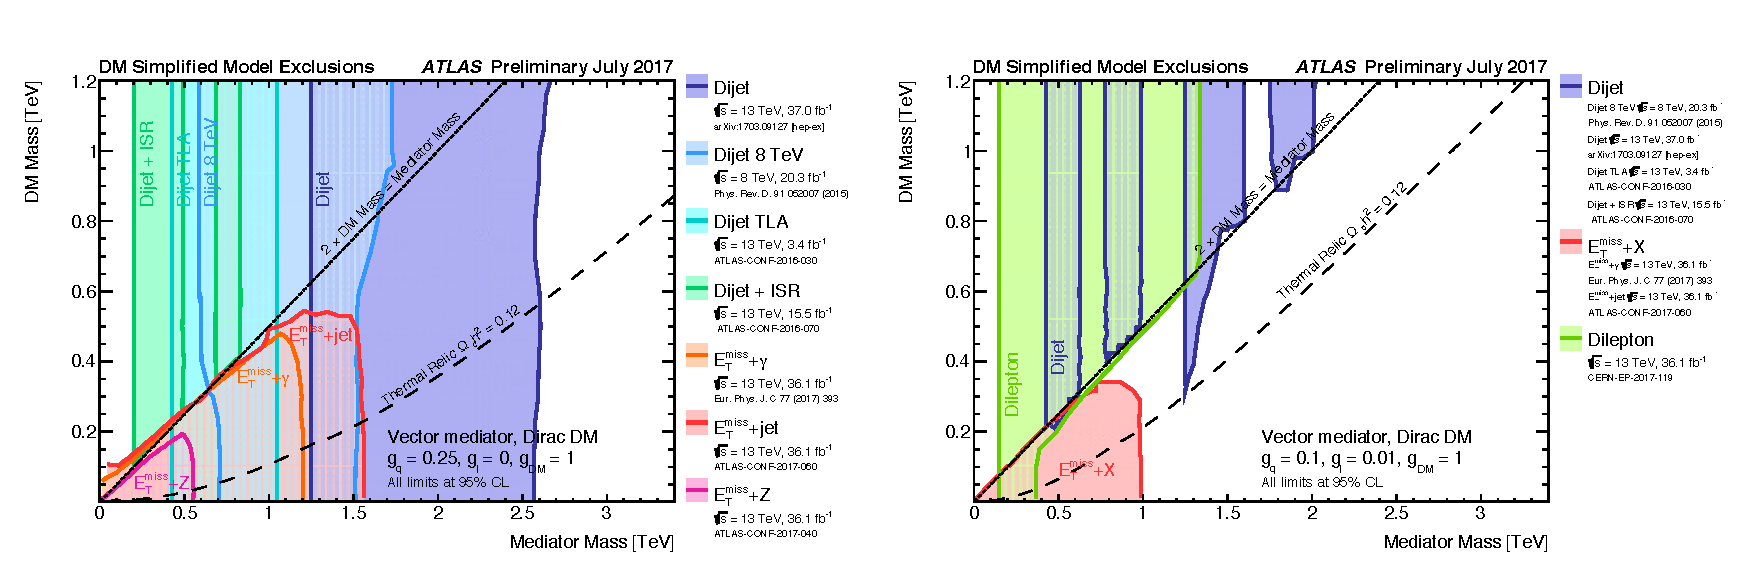
\includegraphics[width=\textwidth]{figures/SummaryPlotsMassMass.pdf}\caption{
Regions in a dark matter mass-mediator mass plane excluded at 95\% CL by a selection of ATLAS dark matter searches, for a vector mediator benchmark model with varying coupling scenarios. Top plots: \gq=0.25, \gl=0.0, \gdm=1.0, axial vector (left, separate search constraints) and vector mediator (right, combined search constraints), highlighting the sensitivity of visible searches in this scenario and the near-equivalence of the vector and axial vector as benchmark models for LHC searches. Bottom plots: \gq=0.1, \gl=0.1, \gdm=1.0 for an axial vector mediator (left) and \gq=0.1, \gl=0.01, \gdm=1.0 for a vector mediator (right), highlighting the sensitivity of the lepton searches and its dependence on the chosen coupling value. Dashed curves labeled "thermal relic" indicate combinations of dark matter and mediator mass that are consistent with a dark matter density of $\omega_c = 0.12 h^2$ and a standard thermal history, as computed in MadDM~\cite{Backovic:2015cra}. The dotted curve indicates the kinematic threshold where the mediator can decay on-shell into dark matter. }
%\gdm=1.0  \gq=0.25universal to all flavors, and a lepton coupling gl set to zero. This choice of couplings corresponds to the "V1" scenario in arXiv:1703.05703. Leptonic decays are absent at tree level. The results use 13 TeV data except for Phys. Rev. D91 052007 (2015). The exclusions from the ATLAS dijet searches are derived from the limits provided on Gaussian-shaped resonances following the procedure recommended by ATLAS in Appendix A of Phys. Rev. D91 052007 (2015) and in arXiv:1703.09127. Small fluctuations in the contour are a product of the dijet reinterpretation scheme. 
%To the left of the curve, annihilation processes described by the simplified model deplete ?c below 0.12 h2. A dotted curve indicates the kinematic threshold where the mediator can decay on-shell into dark matter. The exclusion regions, relic density contours, and unitarity curve are not applicable to other choices of coupling values or model.
\label{fig:sensitivityComparison}
\end{figure}

%CD: if we want coupling-mass, we could show the plots in the figs dir: SummaryPlotsCouplingMass.pdf

%In case sample figure with different scenarios as an example
%\begin{figure}[!htpb]
%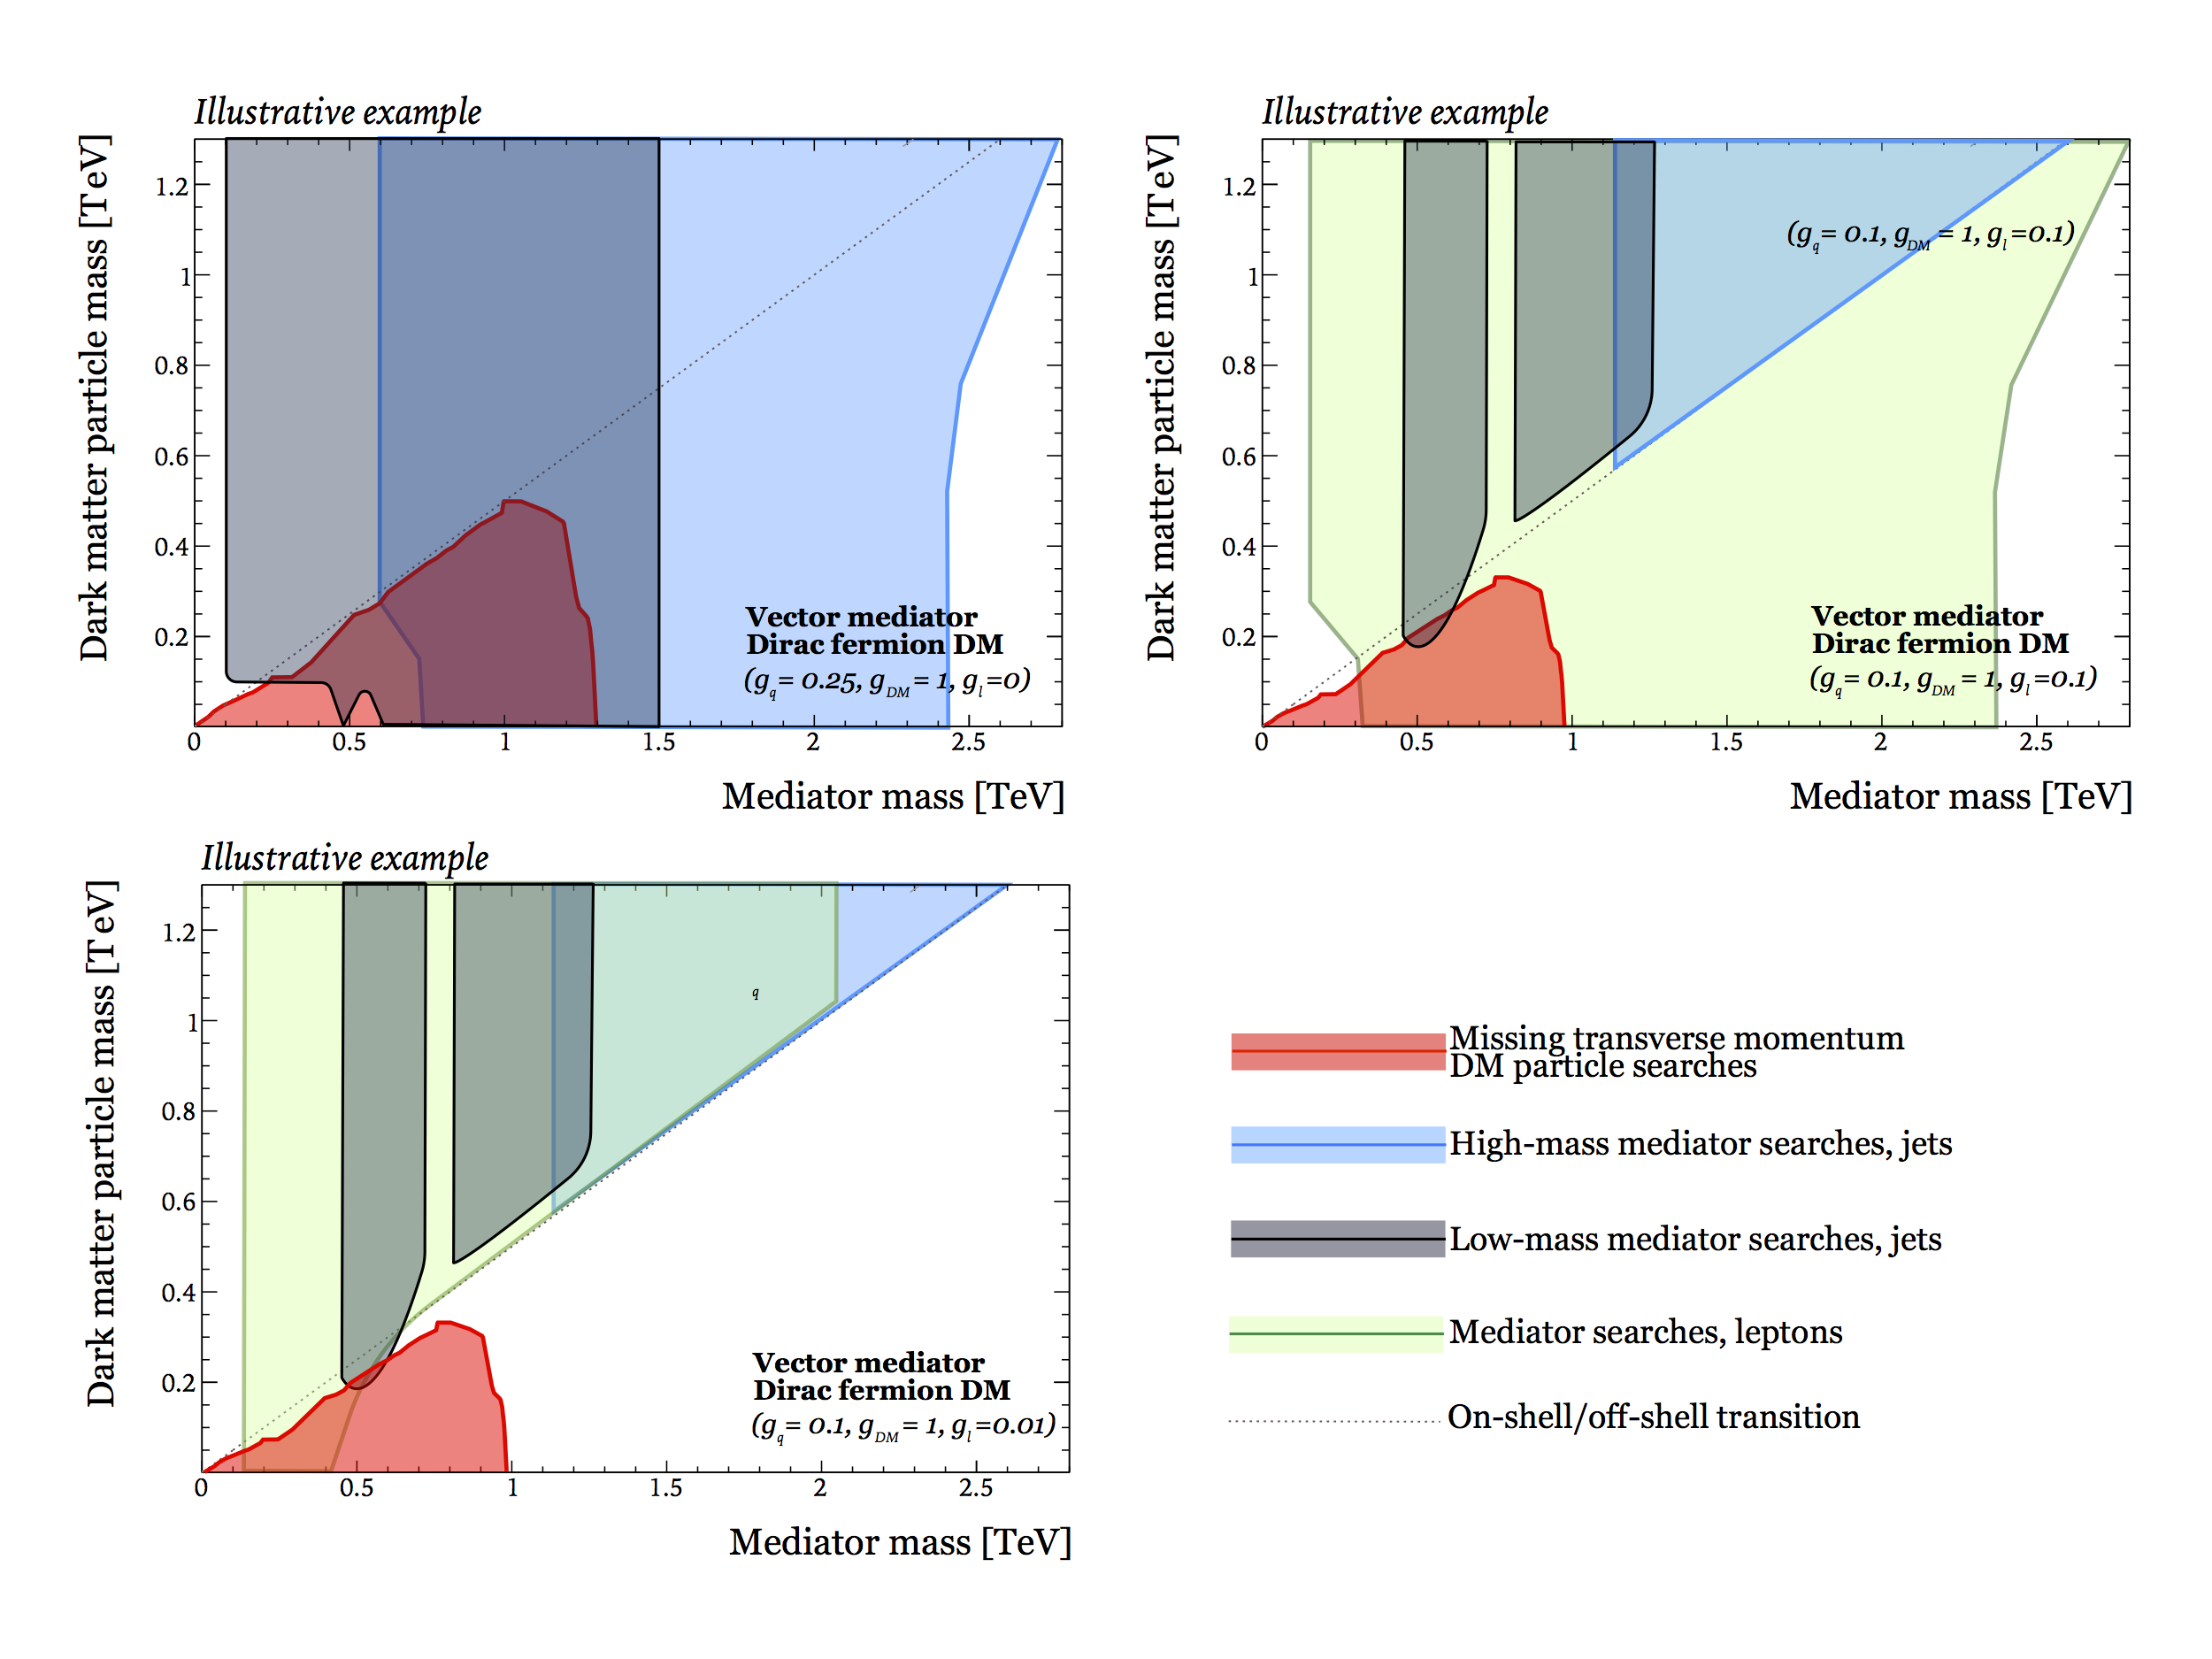
\includegraphics[width=\textwidth]{figures/DMSummary.png}
%\caption{Illustrative examples of the comparison of the sensitivity of searches for visible and invisible mediators in the \mdm-\mmed plane, for different coupling scenarios. No actual data has been used, but experimental observations have been used as inspiration for the figure. From~\cite{AnotherWikipedia}.}
%\label{fig:sensitivityComparison}
%\end{figure}

%It would be nice to make tables of lowest mediator/DM searches+refs for 100 GeV DM mass,
%as a poor-person approximation of a summary plot we can't make because ATLAS data not public. 
 

%%%SUMMARY TABLE FOR MONOX SEARCHES
\begin{table}[h]
\tabcolsep7.5pt
\caption{Summary of searches for BSM mediators at the LHC}
\label{tab:BSMSearchesSummary}
\begin{center}
\begin{tabular}{@{}l|c|c|c|c@{}}
\hline
Signature & Model& \mmed limit & \mdm limit  & Cit.\\
 &  & (\mdm=100 GeV) & (\mmed=100 GeV)  &  \\
%{(}units)$^{\rm a}$ &Head 2 &Head 3 &Head 4 &{(}units)\\
\hline
Jets+\MET & $s-$channel, AV$^{\rm a}$ & Column3 & Column4 & \cite{Sirunyan:2017jix,Aaboud:2017phn} \\
Jets+\MET & $s-$channel, V$^{\rm a}$ & Column3 & Column4 & \cite{Sirunyan:2017jix,Aaboud:2017phn} \\
Jets+\MET & colored scalar & Column3 & Column4 & \cite{Sirunyan:2017jix,Aaboud:2017phn} \\
Photon+\MET & Column 2 & Column3 & Column4 & Column\\
W,Z (had)+\MET 1 & Column 2 & Column3 & Column4 &Column\\
W,Z (lep)+\MET 1 & Column 2 & Column3 & Column4 &Column\\
Higgs+\MET &Column 2 & Column3 & Column4 &Column\\
\hline
\end{tabular}
\end{center}
%\begin{tabnote}
$^{\rm a}$ Coupling values: \gq=0.25, \gdm=1.0; $^{\rm b}$second table footnote.
%\end{tabnote}
\end{table}




\subsection{Searches for SUSY DM}
\label{sec:results_SUSYSearches}

Supersymmetry, besides solving many theoretical problems of the Standard Model, often provides a dark matter candidate. The literature on this subject is far too broad to cover here. Instead, we will broadly sketch progress to date and point out a few areas to watch in the future.

Supersymmetric relic dark matter, the archetype for the WIMP idea, has a long history \cite{doi:10.1016/0550-3213(84)90461-9}. Of these, the most viable and well-studied has been neutralino dark matter. In the Miniminal Supersymmetric Standard Model (MSSM), there are four neutralinos, each a mixture of a wino, a bino, and two higgsino fermion states. The lightest neutralino may be called 'bino-like,' 'wino-like,' or 'higgsino-like' in regions of MSSM parameter space where one of these components dominates the mixture.

The pheno is different depending on the composition, but in general it features MET (the neutralino) plus a lot of X. 
Searches for these things \cite{} (or are discussed in the experimental section).
Talk about differences between different types of dark matter: signature.
One blessing and curse of SUSY is that it is more specific.
An advantage SUSY searches have over searches for 'less-fleshed-out models' is that the signatures are more specific about what comes along with the MET and thus searches can be more directly targeted to particular variants, leading to lower backgrounds etc. than the corresponding inclusive MET+X search. The cost of this advantage is a larger variety of searches that must be done. 
- depends on what cascade decays ultimately produce the LSP.
- spacing between states states in the mass spectrum.
  - NLSP much heavier than LSP: lots of MET
  - narrow spacing NLSP close to LSP mass: low MET (``compressed'')

Higgsino searches nice to find projections for those. going to take a lot of luminosity.

Aside from dark matter comprised of neutralinos, DM could be consistuted from gravitinos. Gravitino DM would not be a thermal relic (because only gravitational strength interactions, cite?). At colliders, it could be produced by the decay of heavier SUSY states. Similar to the neutralino cases, the identity and mass of the heavier states (i.e. the NLSP) determine the signatures, but for the gravitino the favored signatures are different. 
- NLSP could be stop i.e. tops + MET signature
- NLSP could be stau, metastable charged particle at the LHC, relatively long-lived (non-prompt) lepton signatures
- NLSP could be sneutrino and so forth.

%\cite{FengAR} %x-devonthink-item://F9E6F4B6-265D-48CF-B8CC-48B17D28C0DC
%\cite{CraigNN} %

%CD: commented all of this out in favour of three sidebars
%\subsection{Experimental challenges for DM searches at the LHC}
%\label{sec:experimentalChallenges}

%Now that we have seen the searches for invisible particles and their sensitivity to DM models, we will cover the experimental challenges more in detail, as those will be the key to fully exploit %bleurgh
%the Run-2 and Run-3 datasets. 

\subsubsection{pMSSM scans}

To combat the problem of huge number of signatures, the concreteness of SUSY (relative to the [exotics models]) can be put to use. Refs. \cite{10.1140/epjc/s10052-011-1697-z}, and continuing through cite ATLAS (and CMS?) use the so-called pMSSM (define) to define a finite (though large) parameter space to probe, within which one can then ask, systematically, what regions of this parameter space are already excluded by existing results, what regions remain viable, and why those regions have so far remained untouched. This does not necessarily provide rigid or exhaustive exploration of the possibilities, even in the pMSSM as a model, but these efforts may give a coarse-grained map, pointing out what sorts of signatures remain unexplored by current searches. Adding assuptions that relate the LSP to a thermal relic, one can further narrow the list of search targets and key in on particular regions of parameter space for prioritized study (cite battagli etc? and ATLAS paper with relic?). Mention that these assumptions are of course very tenuous, as they deal with physics at potentially much higher energy scales. But DM density is one of the only clues we have about BSM, so more, not less, of this sort of thing is interesting to do (i.e. vary the assumptions).

Other tools to do this. GAMBIT.

\subsection{Searches for DM in association with long-lived particles}
\label{sec:results_LLPSearches}

transition from NLSP talk above (which e.g. could be metastable and long lived) to talking about the exotics/general counterpart to susy.


%%%%%%%%
%ASSORTED JUNK
%%%%%%%%

%beginning with the searches that illustrate many of the experimental 
%
%
% and then signals of MET. 
%
% description has a historical and ordering
%We begin with introducing 
%
%start with introducing the searches, mostly  
%
% of DM searches, we will turn to a [categorization] of the searches done so far. After a summary of searches for interactions through SM bosons, we turn to the experimental results 


%As described in the previous chapter, DM itself is not visible at colliders and has
%to be observed indirectly in association with other visible particles. 
%
%Signals of DM can come from MonoX and diX searches. 
%
%State of the art MC:
%
%Vector and scalar models are known at NLO~\cite{Neubert:2015fka,Haisch:2013ata}
%NLO corrections for vector and scalar models in monoZ and monojet
%
%t-channel
%
%From Millie's talk (see Reaction OmniOutliner):
%Since the DM-mediator-quark vertices allow for simultaneous FS partons with different hard scale, particular prescription needs to be used for the generation of samples with different partons that splits samples in number of mediators. Interference between the diagrams is neglected following Papucci et al. 

%%%Bunch of text from ERC that could be useful for TLA part

%This is what I wrote in ERC, not sure if it's usable

%At the LHC, proton beams with a center of mass energy of 13 \tera\electronvolt \ will collide up to 
%every 25 \nano\second \ at the four interaction points, where experiments are installed. 
%The ATLAS (\textbf{A} \textbf{T}oroidal \textbf{L}HC \textbf{A}pparatu\textbf{S}) experiment 
%is a general purpose detector located at the Interaction Point 1.
%From the Spring of 2010 to Fall 2012 the LHC has recorded a total of 25 \invfb of collision data 
%at 7 and 8 \tera\electronvolt. 
%
%It is the high interaction rate of proton-proton collisions at the LHC that 
%allows the collection of the large dataset necessary to search for rare processes. 
%The design and operation of the ATLAS detector is described in 
%References~\cite{DetectorPaper}. The key subsystems employed in this projects are the calorimeters, 
%where energy deposits from the collimated sprays of particles originated by 
%quarks and gluons are detected. The energy deposits are used as inputs of 
%\textit{jet algorithms}~\cite{Salam:2009jx}: 
%the experimental output used for the analysis is a reconstructed jet that, after calibration, 
%contains information on the kinematics of the original physics process. 
%The system and technologies employed to select and collect interesting data are the crucial components for the 
%innovative Trigger Level Analysis searches outlined in WP2 and WP3, 
%and they are described in more detail in Section~\ref{subsub:datacollection}. 
%
%The LHC will restart operations in Summer 2015, increasing the center of mass energy to 13 TeV. 
%The dataset collected over the course of the planned three years of operations (called \textit{Run 2}, 
%ongoing until mid-2018) corresponds to 100 \invpb~\cite{KEKRossi}. 
%Upgrades to further increase the data rate and the center of mass energy to 14 TeV will be 
%undertaken during the course of 2016, and completed during the 1.5 year technical stop (called LS2).
%LS2 will last until the beginning of 2020, leading to the third LHC run 
%that will collect an additional 200 \invpb of data. 
%
%During LS2, the LHC experiments will undergo major upgrades to their hardware (called Phase-I upgrades). 
%In the final two years of this project that coincide with the LHC Run 3, 
%I will exploit the new gFEX trigger board~\cite{Bartoldus:1602235} to extend the Trigger-Level Analysis 
%method to obtain an increased sensitivity for four-jet final states. 
%
%\subsubsection{Data collection and data analysis in ATLAS at the LHC}
%\label{subsub:datacollection}
%
%The rare signal events sought are buried in an overwhelming number of background events.
%It is therefore necessary to have a \textit{trigger} system that in a very short timescale 
%selects the interesting collision events based on the presence of high transverse momentum physics objects 
%(muons, electrons, photons, jets and tau leptons). 
%
%The ATLAS data collection rate at the end of the trigger selection still
%surpasses other ``Big data'' 
%challenges both in academic research and in industry. 
%As an example, ATLAS and the three other main detectors at the LHC produced and recorded 
%13 petabytes of data just in 2010~\cite{NaturePetabyte}. It is clear
%that with such large dataset new ideas and new analysis techniques are needed,
%especially in the case of small deviations over large backgrounds. 
%One such idea consists of moving the data analysis as close
%to the data taking as possible, ultimately removing the need for storage at all. 
%This proposal moves the first steps for the ATLAS detector in this direction, 
%proposing to only retain a subset of the event information, and eventually 
%to move an entire search to be done in real-time as soon as the data
%is collected. 
%
%\paragraph{The ATLAS Trigger system}
%
%The ATLAS trigger system is subdivided in two levels: Level-1 and High Level Trigger (HLT)
%The first, fast selection is made at L1 using coarse detector information. 
%Its logic is mostly hardwired in the readout electronics, 
%given that the decision needs to be made in less than 2.5 $\mu$ \second. 
%The bandwidth available for data transfer to the HLT and the HLT computing power
%limit the rate that could be accepted by the L1 to 75 kHZ from the initial 40 MHz 
%provided by the LHC~\cite{Sfyrla:1510140}. The events accepted by the L1 trigger 
%are passed on to the HLT trigger, a software subsystem. The longer latency allows 
%to perform a more refined reconstruction of the objects that are used for the selection.
%Jets reconstructed within the HLT system will be called \textit{trigger jets} in the following,
%while \textit{offline jets} are those reconstructed after the event has passed the full trigger chain.
%During the 2012 data taking, ATLAS recorded and reconstructed data at a rate of 
%400 Hz, leaving an additional 200 Hz of recorded data for later reconstruction
%(\textit{delayed} data).  
%
%Since the rate for certain signatures (e.g. multi-jet events that are backgrounds of the 
%searches outlined in this proposal) would saturate the limited bandwidth that needs to be shared 
%by all triggers, some triggers are \textit{prescaled}. 
%This means that only a fraction of the events accepted 
%are effectively passed onto the next level.
%A prescale of 1 means that all events 
%selected by the trigger are accepted, while larger prescales mean that only a fraction 
%1/prescale is accepted. This in turn harms the sensitivity of searches, as signal events
%will be rejected by the trigger system as well. 

%Blurb from ERC

%Hadronic jets are a particularly promising final state for both the Dark Matter mediators 
%produced at the LHC, but also for new, unknown particles that might be created when crossing 
%the threshold of a new energy scale such as in the upcoming LHC run. 
%Not knowing the exact nature of these new particles, it is not possible
%to pin down at which energy scales they are going to be produced, 
%and at which rates. This calls for generic searches that are sensitive 
%to a broad range of theoretical benchmarks, and whose results can be easily
%re-interpreted in different frameworks. The absence of any New Physics discoveries 
%during the first LHC run also points to the need for the study of more elaborate 
%and rare processes that can only be achieved with new analysis techniques. 

%A wide range of theoretical models attempt to incorporate Dark Matter. 
%Many of these models postulate the presence of a new massive subatomic particle
%that interacts only feebly with SM particles as a Dark Matter candidate.
%The presence of these Weakly Interacting Massive Particles (WIMPs) can be inferred in 
%in a variety of experiments. \textit{Direct Detection} 
%experiments detect the interaction between an incoming 
%Dark Matter particle and target nuclei within the detector, by measuring nucleon recoil.
%\textit{Indirect Detection} experiments detect the fluxes of SM particles that 
%are produced from the annihilation of DM particles~\cite{Bertone:2004pz, Bauer:2013ihz}. 
%Dark Matter searches at colliders are supported by the consistency
%of the thermal relic density and the annihilation rates of WIMP candidates with masses
%in the GeV-TeV range, compatible with the energy regime of the LHC~\cite{Bertone:2004pz}. 
%The complementarity of those searches in terms of the WIMP-SM interaction of interest 
%is shown in Figures~\ref{fig:complementarity} (a-c). 
%
%\begin{wrapfigure}{L}{0.7\textwidth}
%% \begin{figure}[!h]
%\centering
%    \includegraphics[width=0.65\textwidth]{figures/SimplifiedModels}
%  \caption[Complementarity of DM searches]{\label{fig:complementarity} Sketch showing the complementarity 
%  between different experiments searching for Dark Matter (a-c). The difference between
%  the EFT approach and the simplified model approach is depicted for collider searches in (c-d).}
%% \end{figure}
%\end{wrapfigure}
%
%Indirect detection experiments such as 
%FERMI~\cite{Hooper:2010mq}, AMS 
%~\cite{PhysRevLett.113.121101} and DAMA~\cite{Bernabei:2003za}
%have observed tantalizing signals 
%with a possible Dark Matter explanation.
%There some tension between direct detection experiments: the signal-like excesses 
%and characteristics of events in the CDMS and CoGENT experiments~\cite{Agnese:2013rvf,Hooper:2010uy}
%are not confirmed by other experiments such as LUX~\cite{Akerib:2013tjd}. 
%
%The flagship searches for Dark Matter at the LHC and at the Tevatron 
%exploit the recoil of undetected pair-produced WIMPs against a jet radiated 
%by one of the initial-state quarks or gluons. Such searches have yet to find 
%evidence for WIMPs (see e.g. Refs. ~\cite{Aad:2013oja,ATLAS:2014wra,Aad:2014vka,Aad:2014vea,Aad:2014tda,ATLAS-CONF-2012-147}
%for the ATLAS Collaboration). 
%
%Results from all these experiments need to be connected in a coherent framework for a 
%successful program of study of Dark Matter in the coming years. 
